\section{Displaying color images}

The image \textit{chairs.jpg} consists of the three different color channels of the RGB spectrum: red, green and blue. Pixel that have a high portion of red color (e.g. the pillows on the chairs) have a very high value in the red color channel. Looking at the greyscale image of this channel, these pixels appear almost white. The very red pillows appear black in the green and blue channel, since their color does not contain a lot of green and blue. Colors that have a almost equal distribution of the three channels are perceived as the range from white, to gray, to black. The image contains mainly white and gray colors, for that reason the three channels look very much alike, as can be seen in figure \ref{fig:task2}.

\begin{figure}[!hbt]
  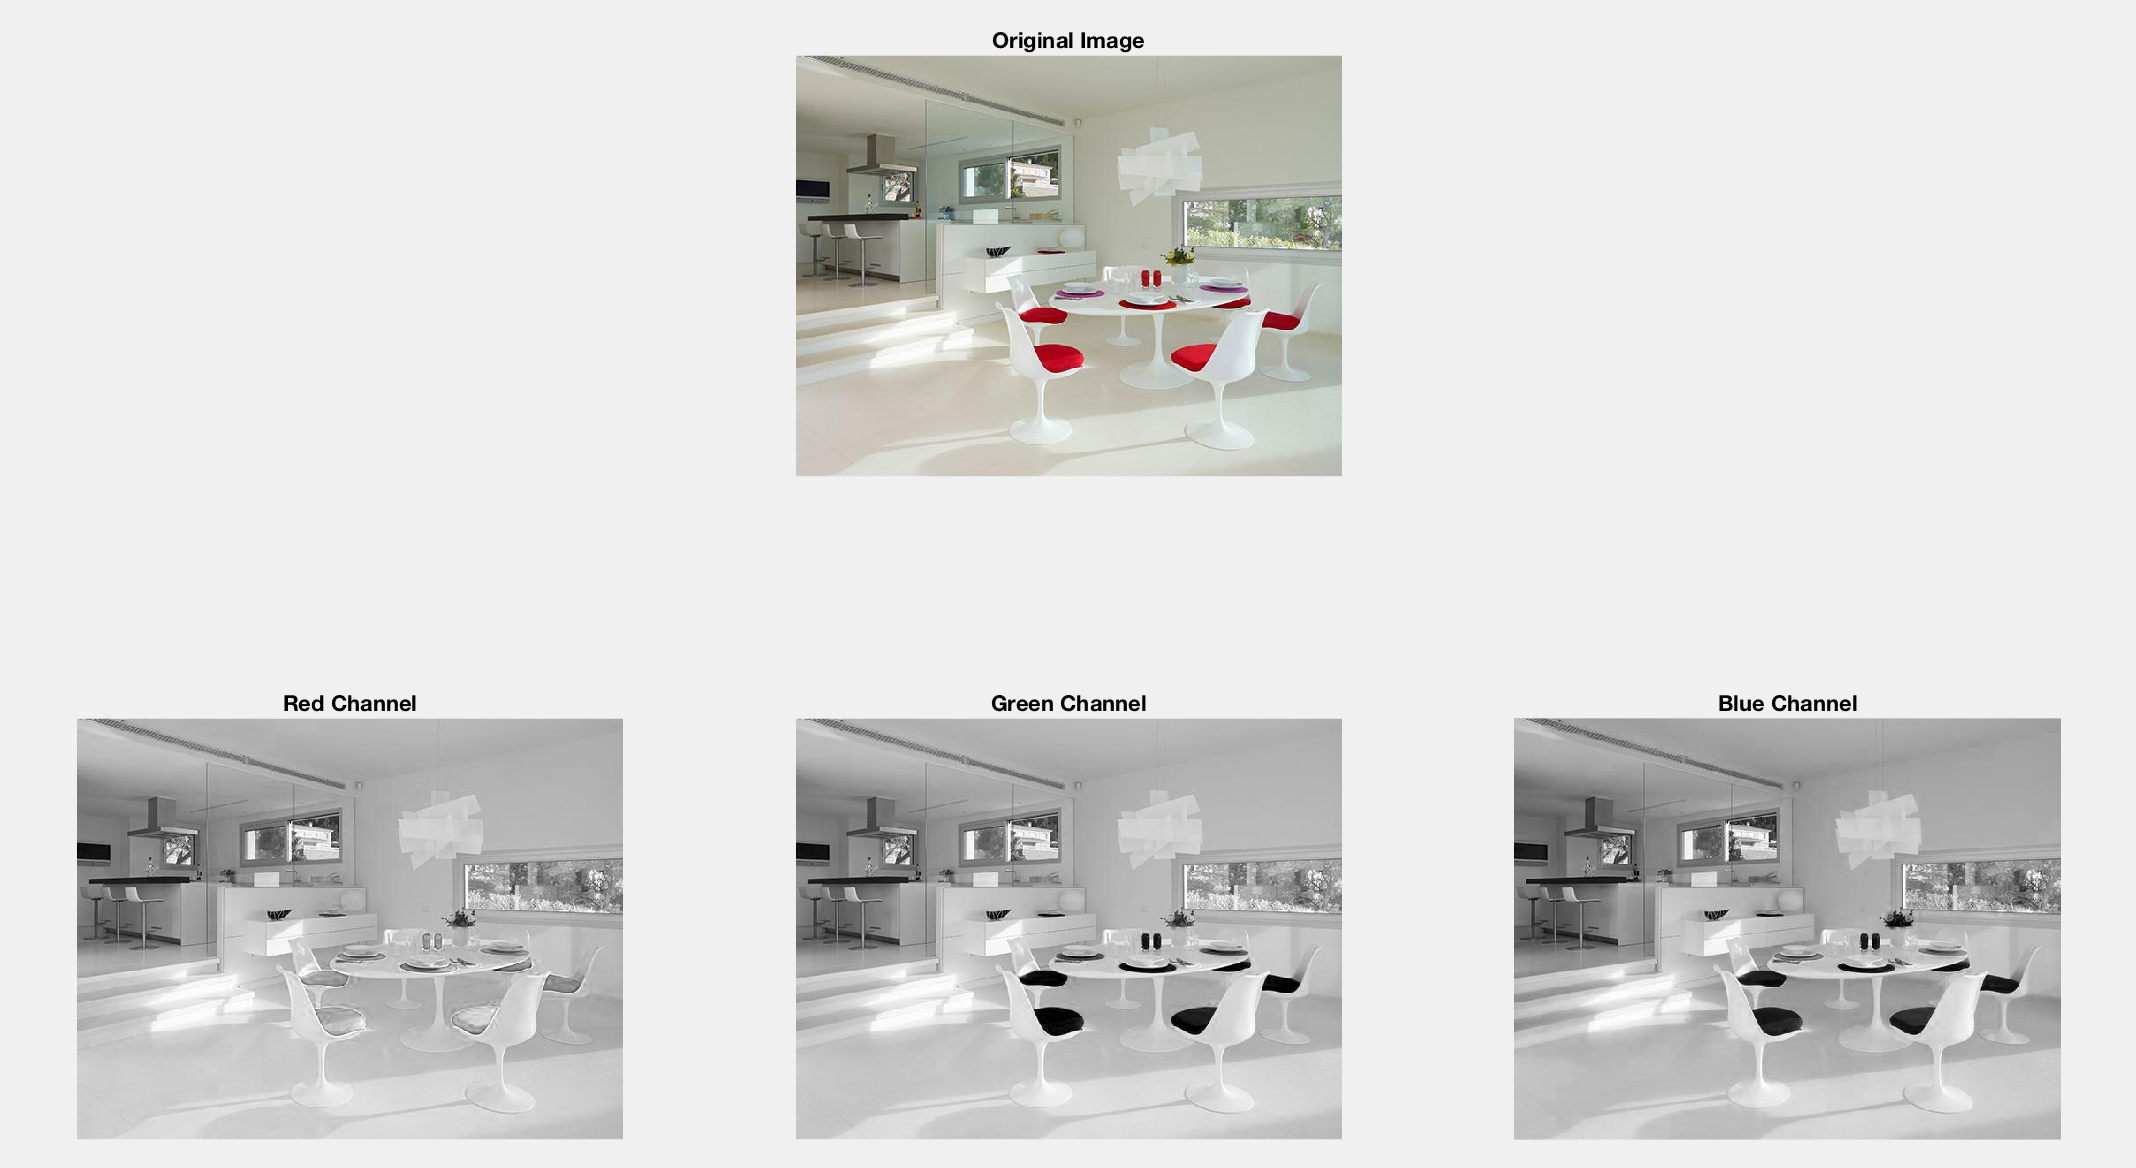
\includegraphics[width=\textwidth]{./img/task2.png}
  \caption{Original Image and its three RGB channels}
  \label{fig:task2}
\end{figure}

It is possible to interchange the different channels with each other. Since there are three channels, 6 different permutations are possible, with one of them being the normal RGB order. The results of those permutations can be seen in figure \ref{fig:task3}.

\begin{figure}[!hbt]
  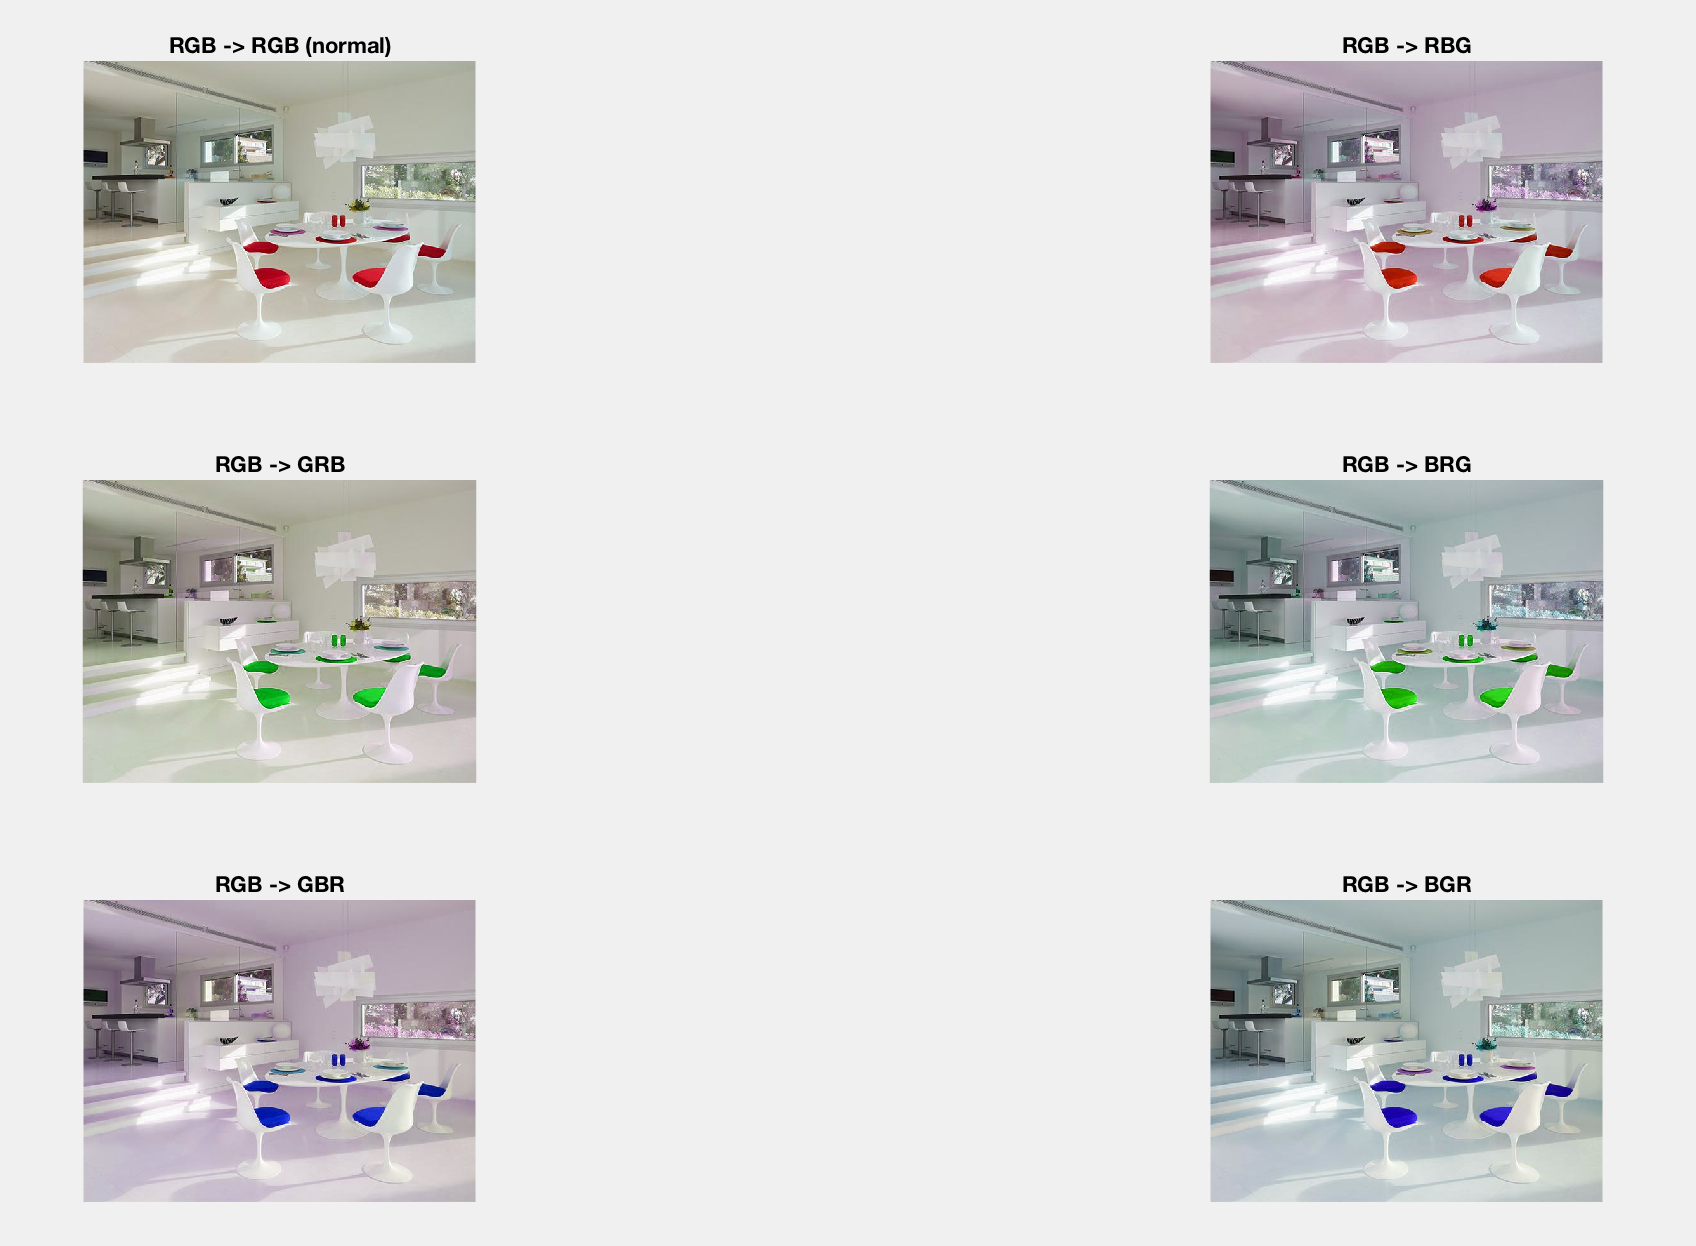
\includegraphics[width=\textwidth]{./img/task3.png}
  \caption{Interchanging the RGB channels}
  \label{fig:task3}
\end{figure}

It is also possible to completely turn off single channels by multiplying all values of a channel by zero. The resulting images are colored in cyan, magenta, and yellow - exactly the colors that are being used in the subtractive color model of printing. The results are shown in figure \ref{fig:task4}.

\begin{figure}[!hbt]
  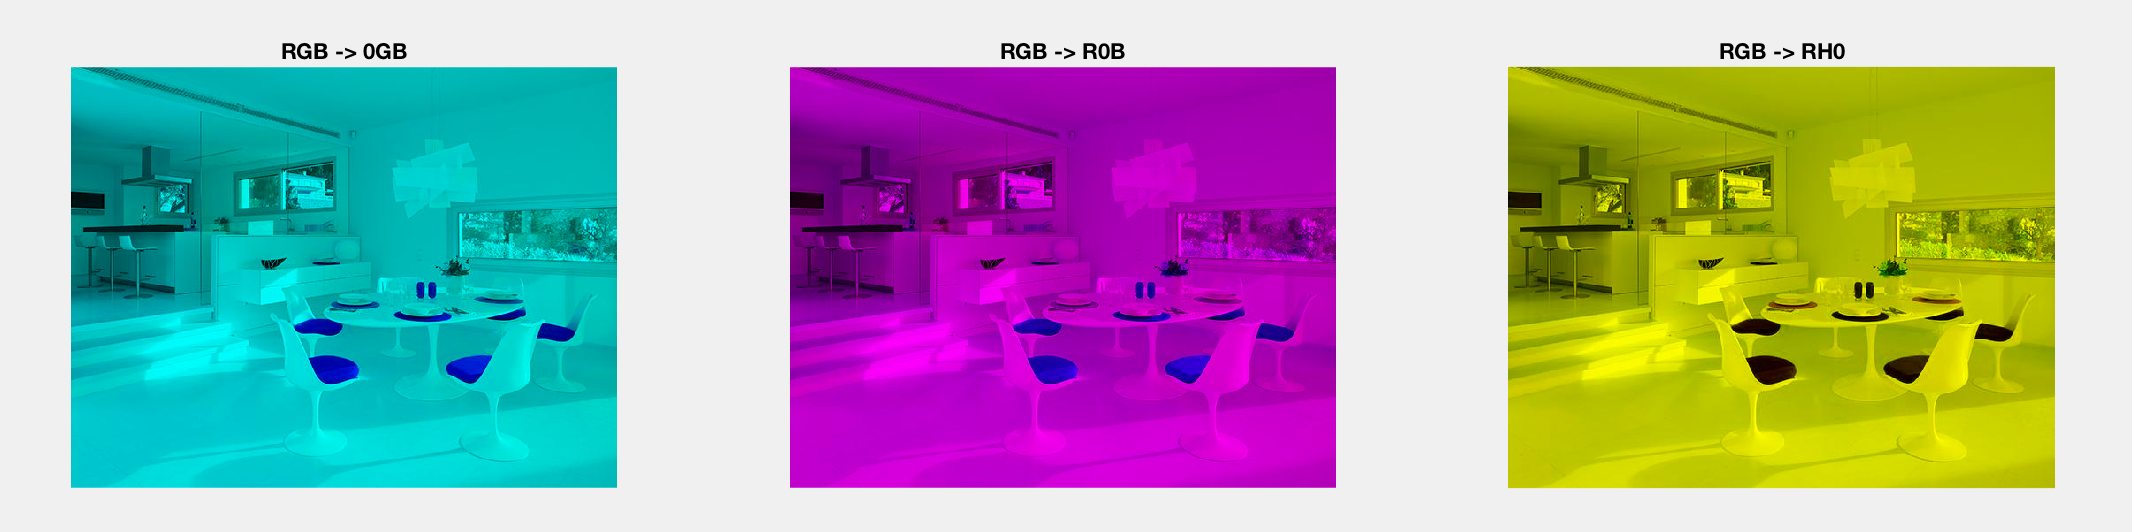
\includegraphics[width=\textwidth]{./img/task4.png}
  \caption{Deactivating single RGB channels}
  \label{fig:task4}
\end{figure}